\newpage

\chapter{Introduction \note{missing}}

\label{chapter:introduction}

Nowadays, computers are invading our daily lives, from work to leisure, from fancy smartphones to an embedded peacemaker that regulates the heartbeat of people.
As human beings, we are known to use tools to enhance our bodies. And thanks to computers, we pushed that step even further, to the point where now we are using machines to extend our brains. Some even argue that one day they will replace us, and therefore we have created our own ending.


from 4.3 exajoules in 2018 to 5.8 exajoules in 2025\footnote{\url{https://www.statista.com/statistics/271139/energy-consumption-of-ict-worldwide}}.
https://www.iea.org/reports/data-centres-and-data-transmission-networks

The Internet of Things (IoT) is one of the most popular topics in computer science and engineering, and it is expected to be a very important part of our lives in the future
However, the energy consumption of ICT equipment is also expected to increase,

Well, this is the problem for the future generations. For the moment, the main concern of humanity is to keep this planet liveable until we find another alternative.
The number of data centers is expected to increase from 1.6 million in 2018 to 2.1 million in 2025, according to [16].

The number of people connected to the Internet has increased by 4.4 billion in 2019, reaching 4.54 billion worldwide, or 59.2\% of the world population, according to the Internet World Stats\footnote{\url{https://www.internetworldstats.com/stats.htm}}.

\begin{figure}
    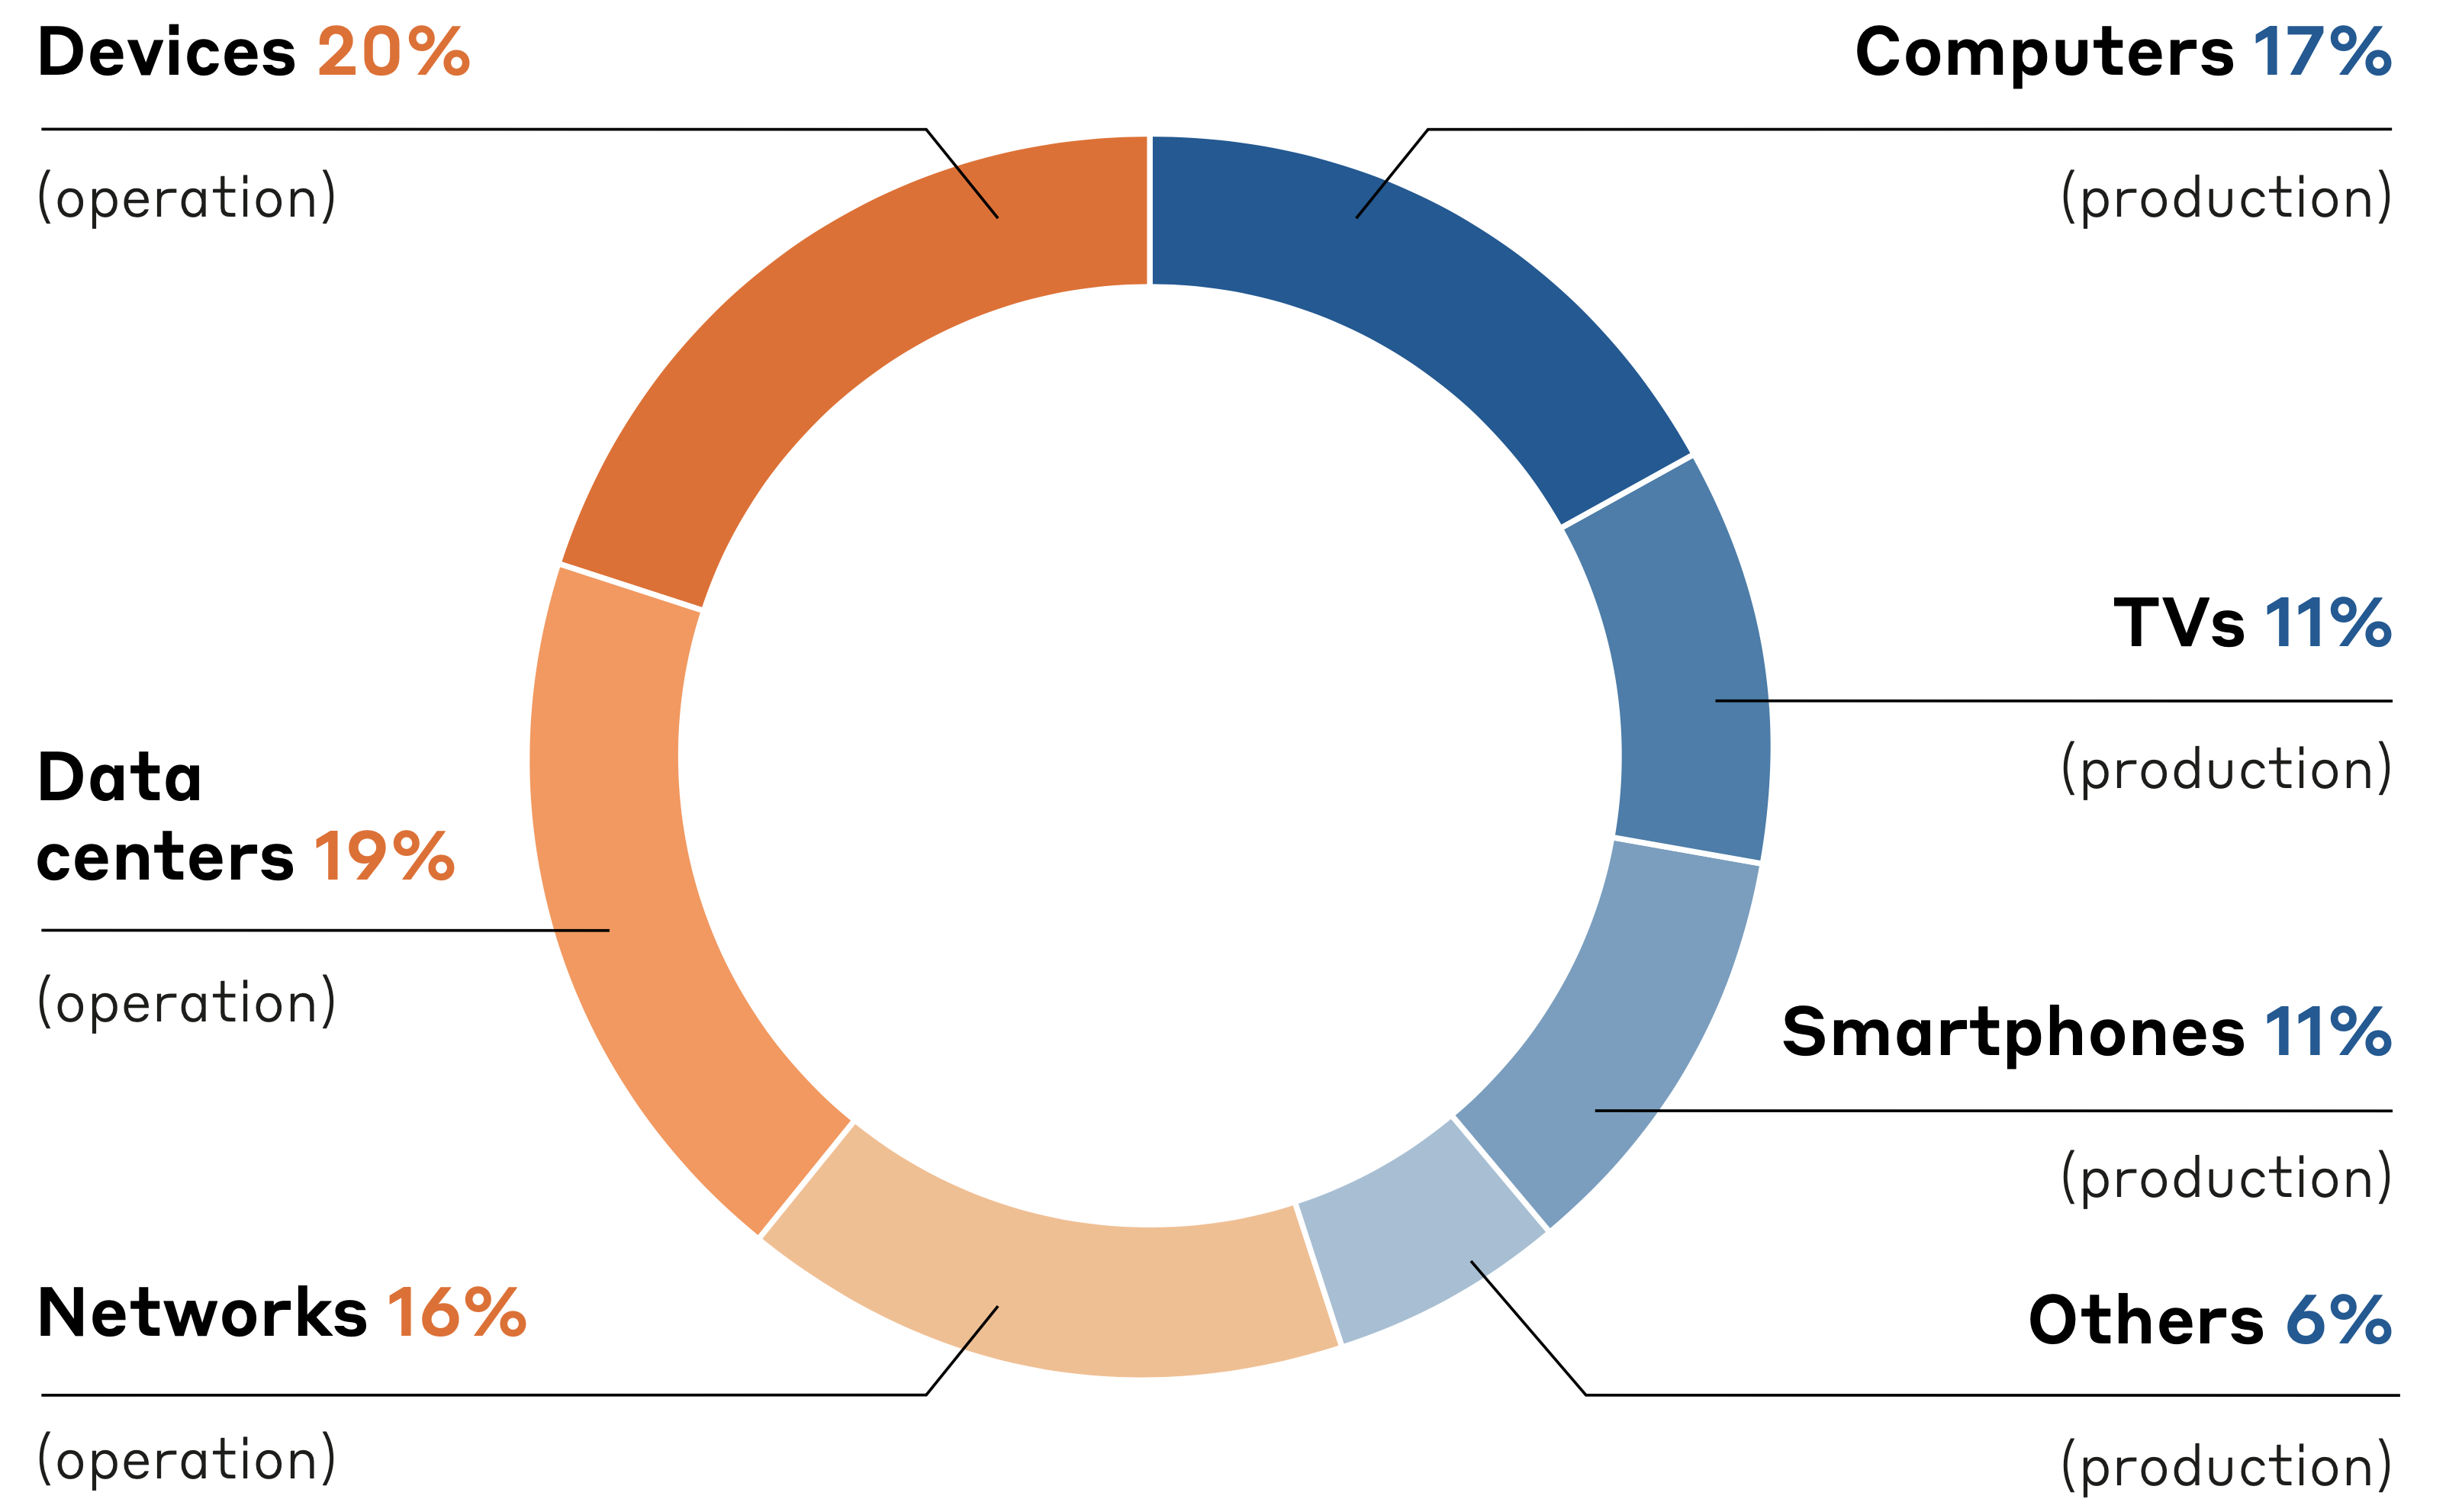
\includegraphics[width=\linewidth]{chapters/distribution_of_ict_consumption.png}
    \caption{Final energy consumption of digital technologies by item in 2017}
    \label{fig:distribution_of_ict_consumption}
\end{figure}

All these new activities have increased the overall environmental footprint of the Information and Communication Technology (ICT) sector, which is estimated to be responsible for approximately 4\% of the greenhouse gaz (GHG) emissions worldwide in 2020 with a worrying 8\% growth rate, according to the French think tank The Shift Project [137], or 2\% according to [13], a similar number to the aviation sector contribution.

    [137]: https://www.theshiftproject.org/article/ict-environmental-impact/

[13]: https://www.theguardian.com/environment/2020/jan/06/tech-industry-emissions-soar-at-double-rate-of-aviation-and-shipping



Unfortunately those machines doesn't help that much. as according to .... ....


Researchers are trying to solve this issue through different angles.
While some scientists are trying to find an alternative green source to generate energy. others focus on reducing this energy consumption.
In computer science we are concerned with the ladder solution %reference.
Therefore most of the works are done on tunning the software and the hardware in order to have a more efficient way use this energy. %more efficient way of producing programs from electricity? 
%say about hardware (i.e. superconductive materials with zero resistance)
In this thesis we are trying to find a way to make the energy consumption of the computer to be as low as possible. %on the software level
%More precisely, the purpose of this thesis is to highlight (attract attention to?) the impact of programers' choices on energy comsumption of software while running the code and to advise them with the strategies to write the greenest possible code.
Our approach is to reduce the energy consumption of the software services by changing certain parameters, such as platform, programming language, and/or the design pattern.

The best way to do so is to formulate a theory behind the energy consumption of algorithm, such as the complexity and the o notation.
Unfortunately this is not possible in the current state of the art. due to the lack of knowledge about the energy consumption of the algorithms, and the strong correlation between this consumption and the hardware configuration.

Unlike algorithm optimization in the field of performance, which is agnostic toward the platform, the energy consumption of the algorithms is dependent on execution environment.
Therefore, for the moment we will start by formulating some hypothesis and explore them using empirical analysis.

Our work will be presented through the following chapters:
\begin{enumerate}
    \item \ref{chapter:literature_review}: Where we discuss the work done on the energy consumption and optimization in software engineering
    \item \ref{chapter:benchmarking}: It will present a set of guidelines and tools to help practitioners measure the energy consumption of their algorithms.
    \item : we will present the impact of programming languages on the energy consumption of the algorithms.
    \item : it will discuss the behaviour of python and the possibile ways to tune it in ordrer to reduce the energy consumpion
    \item : will present a study on java programming language and the impact of the JVM choice on the energy consumpion
    \item : as a prespective we introduce the impact of parallelisme on the enrgy consumption on time agnostic cases
\end{enumerate}




....


\section{Motivation}
....


\section{Research Contributions}


\begin{enumerate}

    \item Introduces
    \item Shows how ....
    \item Proposes ...

\end{enumerate}



\section{Publications}

\begin{enumerate}
    \item ...

    \item ...

    \item ...

\end{enumerate}
\cleardoublepage
